\section{Storyboard}
\label{storyboard}

In this section a storyboard, \autoref{fig:Storyboard}, featuring an ideal use case is shown, along with a short explanation of each pane.//

\begin{enumerate}
\item[\textbf{1}] The bus on the way to the university. 
\item[\textbf{2}] A person is listening to music through their headphones, and drumming along with their fingers.
\item[\textbf{3}] The sound of the drumming is a boring *Bum Bum*
\item[\textbf{4}] The person changes to a different finger but it produces the same boring *Bum Bum*
\item[\textbf{5}] The bus on the way home from the university. 
\item[\textbf{6}] A person is listening to music through their headphones, and drumming along with their fingers.
\item[\textbf{7}] The sound of the drumming is a deep bass-y *Bum Bum*
\item[\textbf{8}] The person changes to a different finger and produces a cool *Tish* -sound
\end{enumerate}


\begin{figure}[H]
\centering
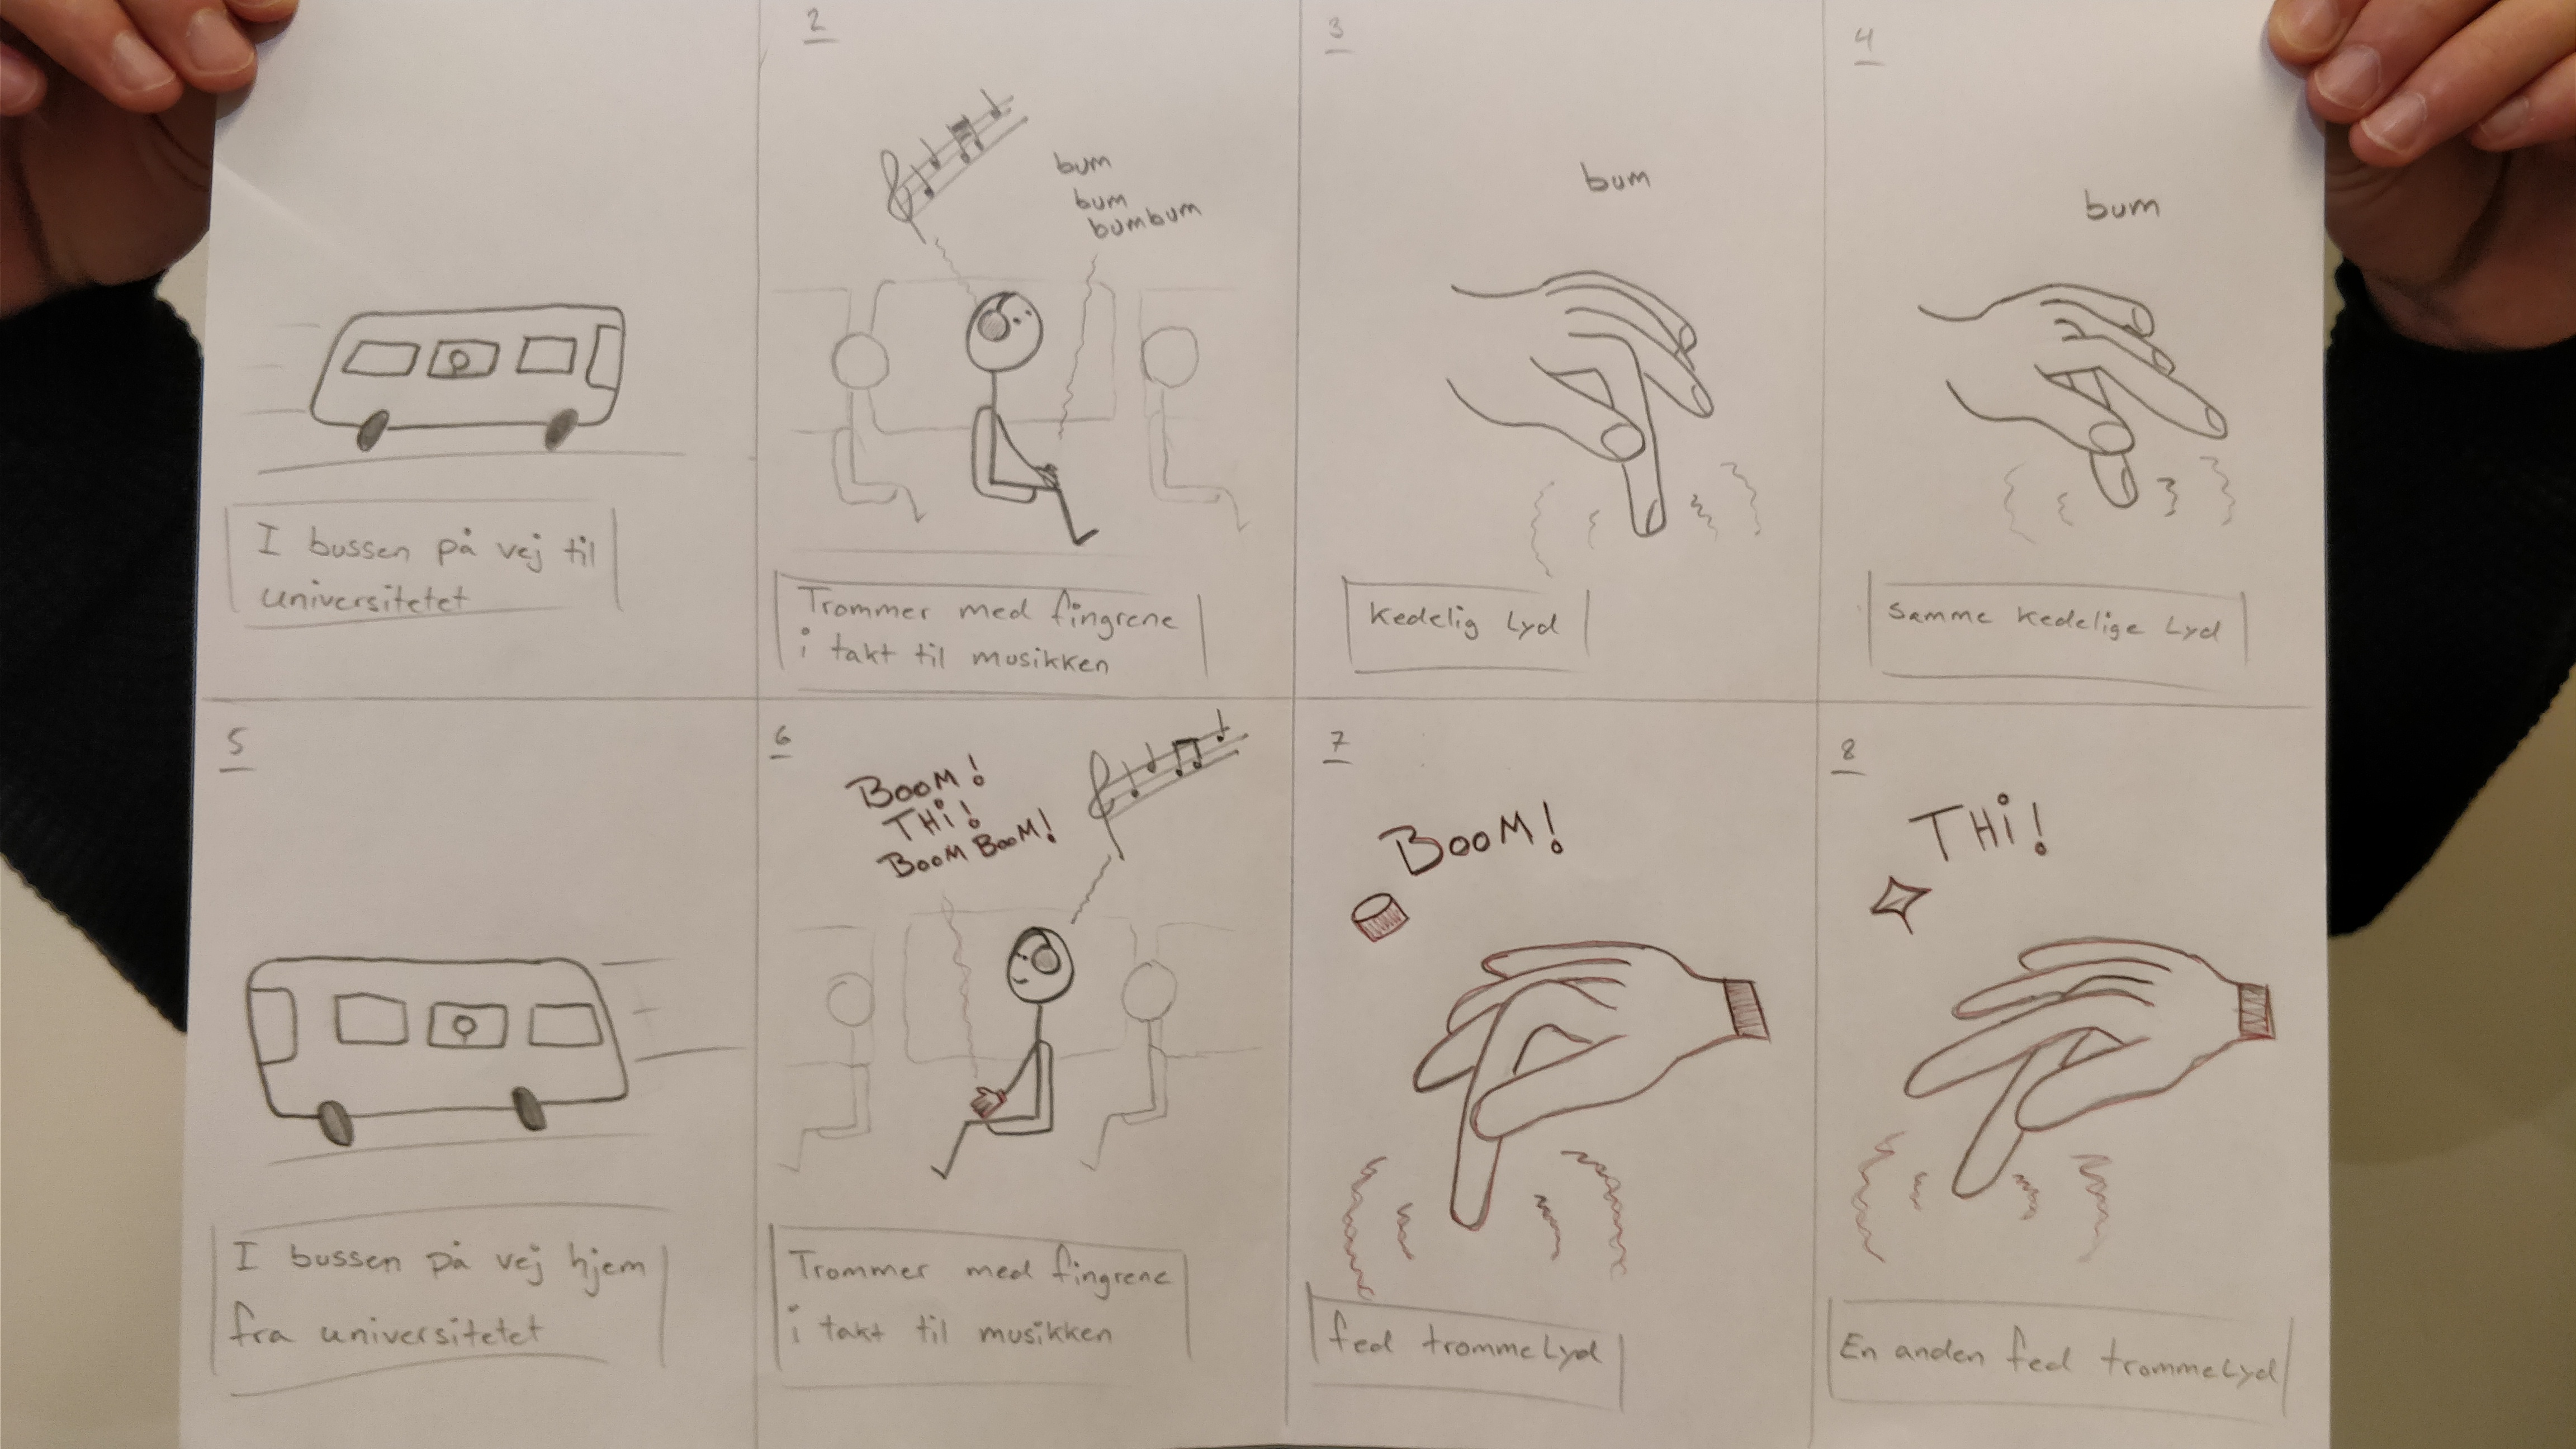
\includegraphics[width = \textwidth]{Figure/Billeder/IMG_20171114_121225.jpg}
\caption{Storyboard for a specific use case.}
\label{fig:Storyboard}
\end{figure}